\documentclass[a4paper, 12pt, titlepage]{article}
\usepackage[utf8]{inputenc}
\usepackage[english]{babel}
\usepackage[]{parskip}
\usepackage{graphicx}
\usepackage{xcolor}
\usepackage{paralist} % compactitem
\usepackage{csquotes}
\usepackage{wrapfig}
\usepackage{subfig}
\usepackage{csvsimple} % csv tables
\usepackage{caption} % ContinuedFloat macro

% Title spacing
\usepackage{titlesec}
\titlespacing*{\section}{0pt}{0pt}{0pt}
\titlespacing*{\subsection}{0pt}{-5pt}{-5pt}
\titlespacing*{\subsubsection}{0pt}{0pt}{0pt}

% Citations
\usepackage[
  style=ieee,
  citecounter,
  labelnumber,
  backend=biber,
  bibencoding=utf8,
  sorting=none
]{biblatex}
\addbibresource{references.bib}

% Code blocks
\usepackage{listings}
\definecolor{codegreen}{rgb}{0,0.6,0}
\definecolor{codegray}{rgb}{0.5,0.5,0.5}
\definecolor{codepurple}{rgb}{0.58,0,0.82}
\definecolor{backcolour}{rgb}{1.0,1.0,1.0}
\lstdefinestyle{mystyle}{
  backgroundcolor=\color{backcolour},
  commentstyle=\color{codegreen},
  keywordstyle=\color{magenta},
  numberstyle=\tiny\color{codegray},
  stringstyle=\color{codepurple},
  basicstyle=\ttfamily\tiny,
  breakatwhitespace=false,
  breaklines=true,
  captionpos=b,
  keepspaces=false,
  numbersep=5pt,
  showspaces=false,
  showstringspaces=false,
  showtabs=false,
  tabsize=2
}
\lstset{style=mystyle}

% Custom commands
% Referencing
\newcommand{\figRef}[1]{Figure \ref{#1}}
\newcommand{\tabRef}[1]{Table \ref{#1}}
\newcommand{\eqRef}[1]{(\ref{#1})}
% Values
\newcommand{\digitwidth}{0.08\textwidth}
\newcommand{\doubledigitwidth}{0.15\textwidth}

\title{EECE6036 - Homework 5}
\author{Wayne Stegner}
\date{\today}

\begin{document}
  \maketitle
  \section{Problem 1}
  \subsection{Problem Summary}
  \par The goal of this problem is to create a self-organized feature map
  (SOFM).
  The SOFM will have a 12 X 12 neuron output map, and it will learn the
  features of the MNIST dataset.

  \subsection{Results}
  \subsubsection{System Description}
  \par \tabRef{tab:sofm_param} shows the hyper-parameters used in training the
  SOFM.
  These hyper-parameters were found empirically with considerations for
  maximizing the classification accuracy for the second problem of this
  assignment.
  \begin{table}[htb]
    \centering
    \caption{Autoencoder Training Hyper-Parameters}
    \csvautotabular{data/sofm_param.csv}
    \label{tab:sofm_param}
  \end{table}
  \par Weight initialization is done on a uniform distribution on the interval
  $(0, 1)$.
  \par This SOFM trains using two-phase learning, as described in the slides.
  In the first phase, the learning rate, $\eta(t)$ starts at $\eta_{0}$, and it
  decays to $\eta_{floor}$ by:
  \begin{center}
    \par $\eta(t) = \eta_{0} * exp(\frac{-t}{\tau_{L}})$
  \end{center}
  \begin{center}
    \par $\tau_{L} = \frac{-epochs_{phase\_1}}{ln(\eta_{floor} / \eta_{0})}$
  \end{center}
  \par Similarly, the neighborhood parameter, $\sigma(t)$ starts at
  $\sigma_{0}$, and it decays to $\sigma_{floor}$ by:
  \begin{center}
    \par $\sigma(t) = \sigma_{0} * exp(\frac{-t}{\tau_{N}})$
  \end{center}
  \begin{center}
    \par $\tau_{N} = \frac{-epochs_{phase\_1}}{ln(\sigma_{floor} / \sigma_0)}$
  \end{center}
  \par During the second phase, the learning rate and neighborhood parameter
  are held at $\eta_{floor}$ and $\sigma_{floor}$ respectively.

  \subsubsection{Heat Maps}
  \par \figRef{fig:heatmap} shows activation heat maps for the test set after
  training.
  These maps were found by measuring the number of times a given neuron won for
  each class.

  \subsubsection{Features}
  \par \figRef{fig:feat} shows the feature map learned by the SOFM after
  training.
  Each feature is a representation of the weights for that neuron.

  % Float Pages
  \begin{figure}[p]
    \centering
    \subfloat{
      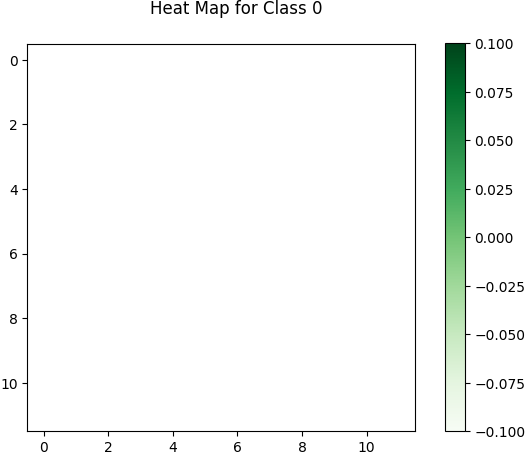
\includegraphics[width=0.45\textwidth]
        {images/heatmaps/class_0.png}
    }
    \subfloat{
      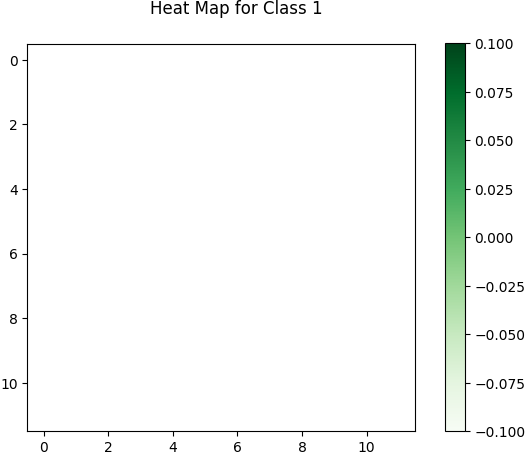
\includegraphics[width=0.45\textwidth]
        {images/heatmaps/class_1.png}
    } \\
    \subfloat{
      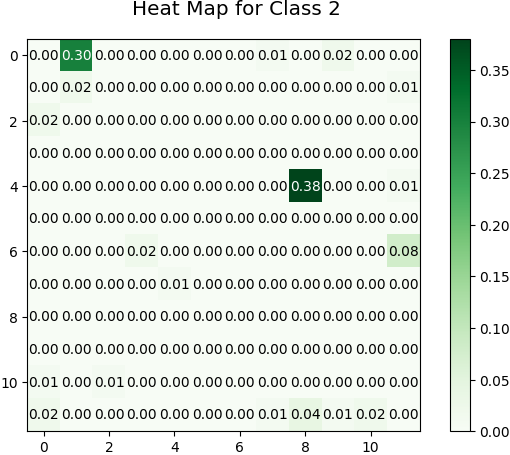
\includegraphics[width=0.45\textwidth]
        {images/heatmaps/class_2.png}
    }
    \subfloat{
      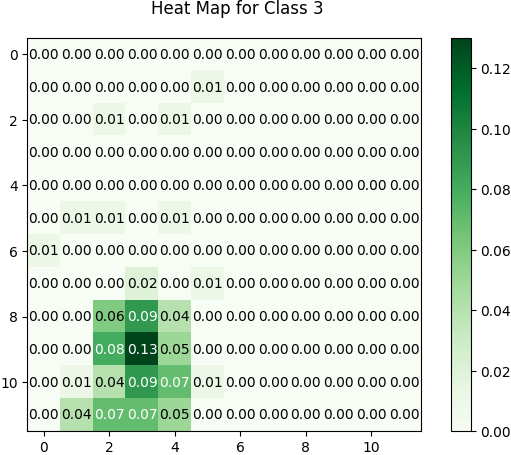
\includegraphics[width=0.45\textwidth]
        {images/heatmaps/class_3.png}
    } \\
    \subfloat{
      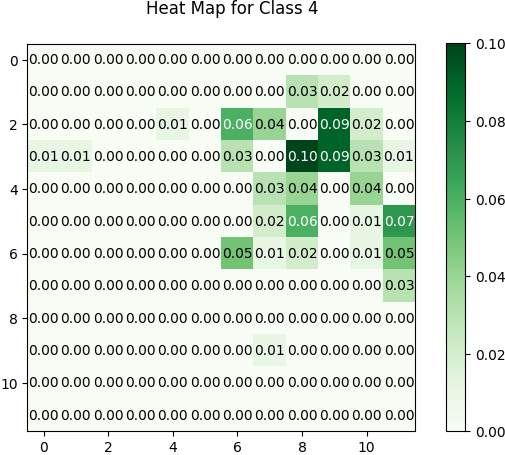
\includegraphics[width=0.45\textwidth]
        {images/heatmaps/class_4.png}
    }
    \subfloat{
      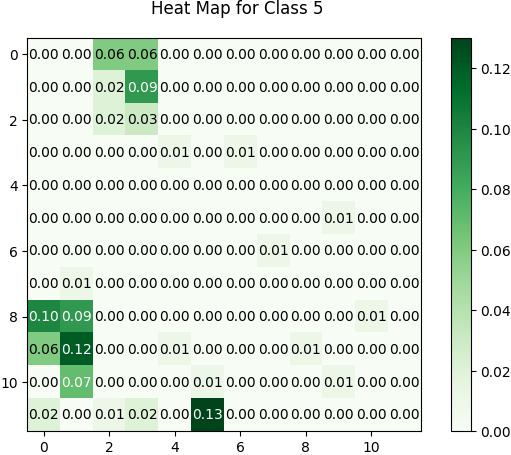
\includegraphics[width=0.45\textwidth]
        {images/heatmaps/class_5.png}
    }
    \caption{Class heat maps of the SOFM.}
    \label{fig:heatmap}
  \end{figure}
  \begin{figure}[p]\ContinuedFloat
    \centering
    \subfloat{
      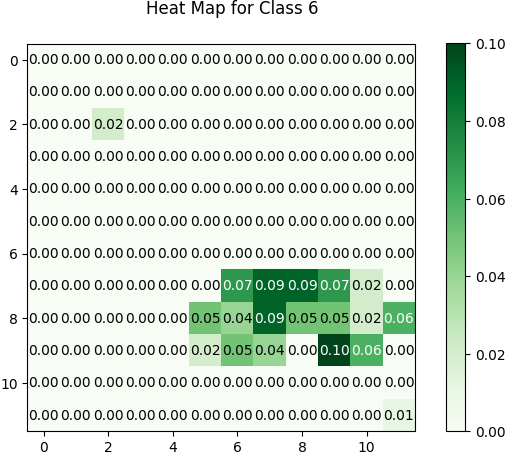
\includegraphics[width=0.45\textwidth]
        {images/heatmaps/class_6.png}
    }
    \subfloat{
      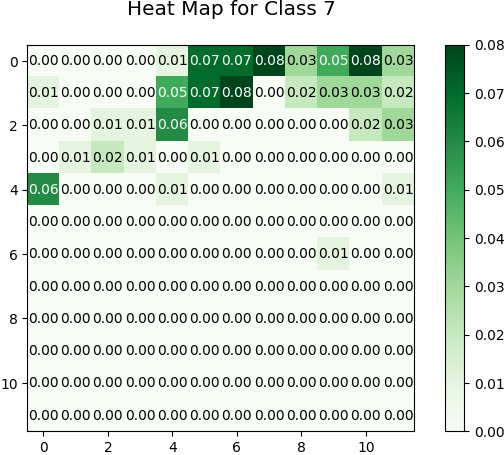
\includegraphics[width=0.45\textwidth]
        {images/heatmaps/class_7.png}
    } \\
    \subfloat{
      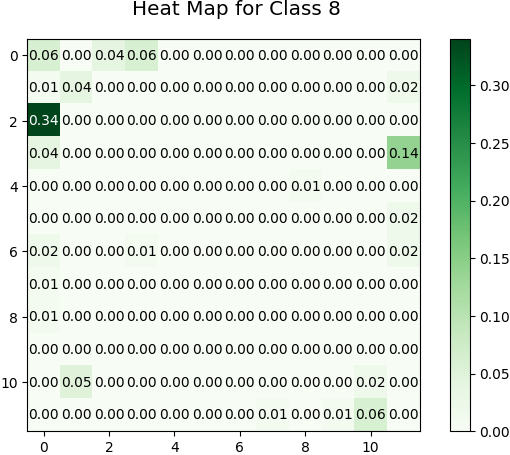
\includegraphics[width=0.45\textwidth]
        {images/heatmaps/class_8.png}
    }
    \subfloat{
      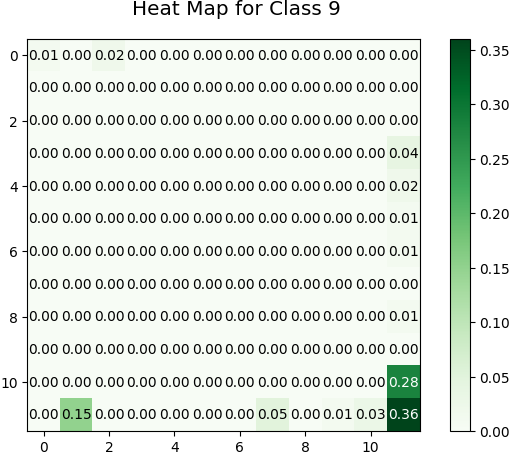
\includegraphics[width=0.45\textwidth]
        {images/heatmaps/class_9.png}
    }
    \caption{Class heat maps of the SOFM, continued.}
    \label{fig:heatmap_cont}
  \end{figure}
  \begin{figure}[p]
    \centering
    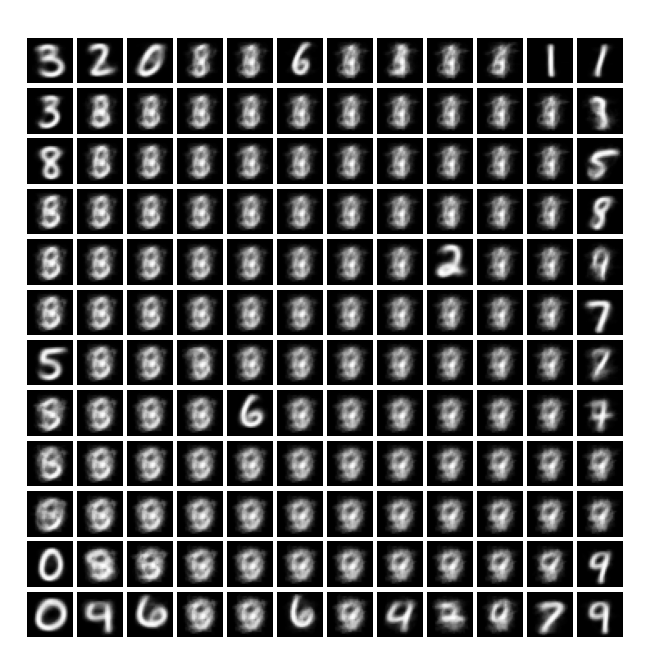
\includegraphics[width=0.5\textwidth]{images/features.png}
    \caption{Feature map produced by the SOFM algorithm.}
    \label{fig:feat}
  \end{figure}

  \subsection{Discussion and Analysis of Results}
  \par Overall, the results look pretty good.
  The class heat maps in \figRef{fig:heatmap} show that the classes each have
  their own distinct regions of activity, with a few exceptions.
  These regions of activity correlate with the class appearing on the feature
  map.
  For example, the heat map for class 0 is active in the bottom right corner,
  and the feature map in \figRef{fig:feat} looks like 0s in the bottom right
  corner.
  Classes 4 and 9 are very close in proximity, with class 4 being in the
  middle of the class 9 region.
  This is expected because 4 and 9 look very similar, so their regions on the
  feature map should be spatially close together.
  The feature map in \figRef{fig:feat} supports this observation.
  In the upper right portion of the feature map, there is a mix of 4s and 9s in
  a similar arrangement to the heat maps for those classes.
  Also in \figRef{fig:heatmap}, the heat map for class 5 shows three major
  regions of activity.
  The feature map in \figRef{fig:feat} has 5s appearing in those regions.
  \par Classes which are similar in shape are spatially close to each other in
  the feature map.
  For example, the bottom left corner of the feature map in \figRef{fig:feat}
  has a combination of 3s and 5s because they are similar in shape.
  Both 3 and 5 are similar to 8, which is found directly above the 3s and 5s in
  the feature map.
  6 and 0 are also similar, and 6 is found just above the 0 region in the
  feature map.
  \par There are a few features in \figRef{fig:feat} which do not clearly
  resemble any class.
  For example, the feature three blocks down and three from the left side looks
  like a smudge or a blur.
  That same feature exhibits activity in the heat maps in \figRef{fig:heatmap}
  in classes 2, 3, 5, 6, 7, and 8.
  That feature may be an artifact of the hyper-parameters chosen for training,
  and more testing should be done to try to eliminate ambiguous features.

  \subsection{Conclusion}
  \par The SOFM is able to effectively learn features from the MNIST dataset
  and group them by similarity.
  Further optimizing the hyper-parameters of the network may help to improve
  the produced feature map further.

  \pagebreak
  \section{Problem 2}
  \subsection{Problem Summary}
  \par The goal of this problem is to create a classifier using the features
  learned from the SOFM trained in Problem 1.
  This is done by passing the image through the SOFM using winner-take-all to
  generate a one-hot encoded feature vector to pass into the MLP classifier.

  \subsection{Results}
  \subsubsection{System Description}
  \par \tabRef{tab:class_param} shows the hyper-parameters used in training the
  classifier.
  These hyper-parameters were found empirically.
  \begin{table}[htb]
    \centering
    \vspace{-12pt}
    \caption{Classifier Training Hyper-Parameters}
    \vspace{-12pt}
    \csvautotabular{data/class_params.csv}
    \label{tab:class_param}
    \vspace{-12pt}
  \end{table}
  \par This network uses the same training algorithm as the previous problems,
  including momentum, thresholding, early stopping, and weight decay.

  \subsubsection{Network Results}
  \par Throughout the duration of training, the loss of the training and
  validation sets was tracked every 5 epochs, shown in \figRef{fig:loss}.
  The vertical lines designate the point where the validation error is
  minimized.
  The classifier achieves a minimal test loss of
  \input{data/test_loss.dat}\unskip{} at epoch
  \input{data/best_epoch.dat}\unskip{}.
  \begin{figure}[htb]
    \centering
    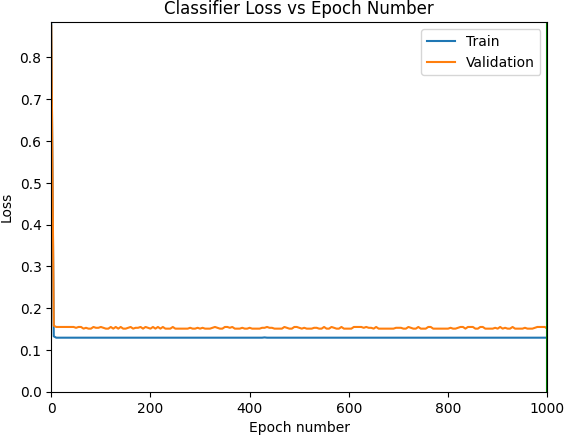
\includegraphics[width=0.5\textwidth]{images/loss_graph.png}
    \caption{Training and validation loss of the classifier.}
    \label{fig:loss}
  \end{figure}
  \par \figRef{fig:conf} show the confusion matrices for the train and
  test sets of the classifier.
  \begin{figure}[htb]
    \centering
    \subfloat{
      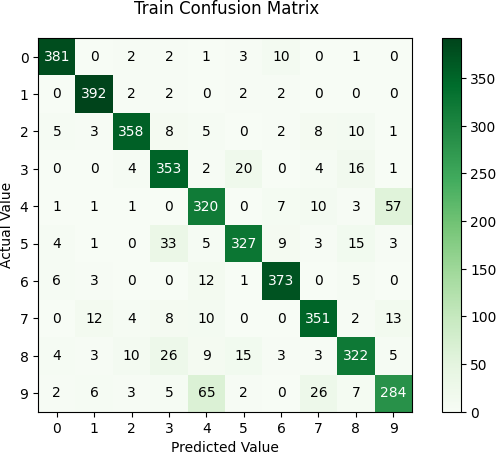
\includegraphics[width=0.45\textwidth]
        {images/train_conf_mat.png}
      \label{fig:conf_train}
    }
    \subfloat{
      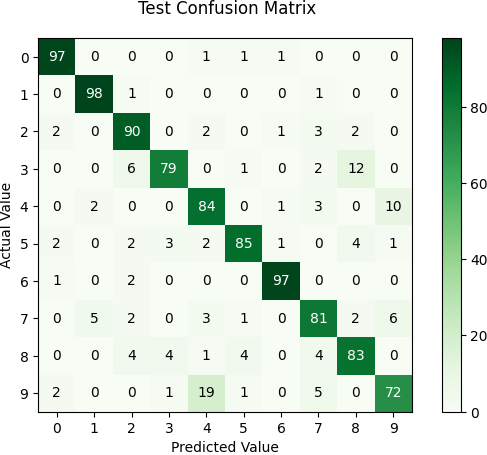
\includegraphics[width=0.45\textwidth]
        {images/test_conf_mat.png}
      \label{fig:conf_test}
    }
    \caption{Confusion matrices of the classifier.}
    \label{fig:conf}
  \end{figure}

  \subsection{Discussion and Analysis of Results}
  \par Overall, the classifier performs pretty well.
  The network only took 50 epochs to train, and was able to train significantly
  faster than the previous classifiers.
  The confusion matrices in \figRef{fig:conf} show a dark diagonal line but
  with some visible confusion, especially between classes 4 and 9.
  The significant points of confusion are between classes which are adjecent,
  such as 4/9 and 3/8.
  \par The classification performance was not as good as the classifiers from
  Homework 3 (loss = 0.070) and Homework 4 (losses of 0.103 and 0.121).
  It makes sense that this classifier is not as performant, because the one-hot
  vectors from the SOFM do not carry as much information as the analog layers
  from the MLPs.

  \subsection{Conclusion}
  \par Using the features learned by the SOFM, the classifier is able to
  effectively classify the MNIST dataset.
  While its performance is not as good as the previously studied classifiers,
  it effectively demonstrates how the SOFM features are viable for
  distinguishing between different digits.

\end{document}
